\documentclass[tikz,crop,convert={density=200,outext=.png},border=0.4cm]{standalone}

\usetikzlibrary{matrix}
\usepackage{pgfplots}
\usepackage{amsmath}
\usetikzlibrary{arrows.meta}
\usepackage{physics}
\usepackage{xcolor}
\definecolor{green_1}{RGB}{0,68,27}
\definecolor{green_2}{RGB}{35,139,69}
\definecolor{green_3}{RGB}{102,194,164}
\definecolor{green_4}{RGB}{140,150,198}

% Colours for the time domain
\definecolor{red_1}{RGB}{103,0,31}
\definecolor{red_2}{RGB}{206,18,86}
\definecolor{red_3}{RGB}{2,56,88}
\definecolor{red_4}{RGB}{5,112,176}
% Colours for the phase plane
\definecolor{blue_1}{RGB}{2,56,88}
\definecolor{blue_2}{RGB}{4,90,141}
\definecolor{blue_3}{RGB}{5,112,176}
\definecolor{blue_4}{RGB}{54,144,192}
% Colours for the text
\definecolor{He}{RGB}{103,0,31}
\definecolor{Mi}{RGB}{206,18,36}
\definecolor{To}{RGB}{231,41,138}

\pgfplotsset{compat=newest,
    width=10cm,
    %height=3cm,
    scale only axis=true,
    max space between ticks=25pt,
    try min ticks=5,
    every axis/.style={
        axis y line=left,
        axis x line=middle,
        axis line style={thick,->,>=latex, shorten >=-.3cm}
    },
    every axis plot/.append style={thick},
    tick style={black, thick},
}
\tikzset{
    semithick/.style={line width=0.8pt},
}
\usepgfplotslibrary{groupplots}
\usepgfplotslibrary{dateplot}
% Document begins
\begin{document}
% =========================================================================================================
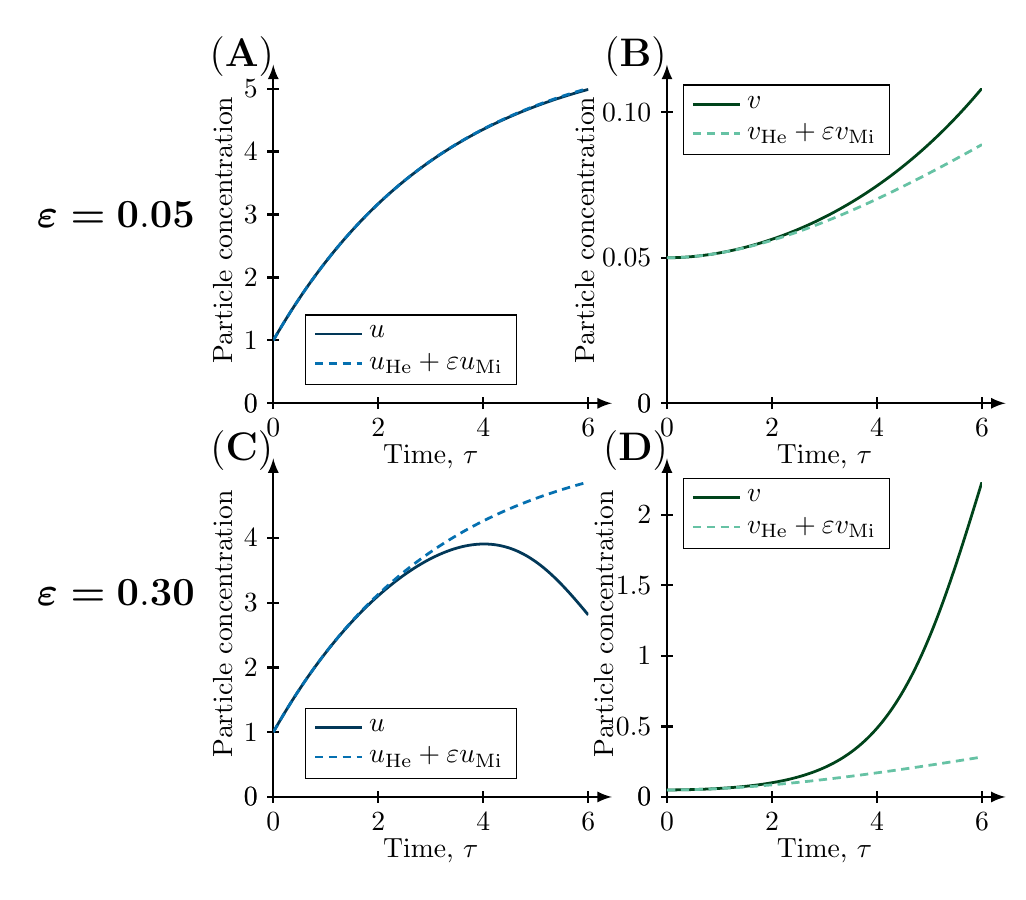
\begin{tikzpicture}
    \begin{axis}[name=plot1,height=4cm,width=4cm,xlabel={Time, $\tau$},ylabel={Particle concentration},ymin = {0},x label style={at={(axis description cs:0.5,-0.1)},anchor=north},y label style={at={(axis description cs:-0.1,0.55)},rotate=0,anchor=south},extra x ticks = {0}, extra y ticks= {0},legend style={at={(axis description cs:0.1,0.17)},anchor=west,nodes={scale=1.0, transform shape}},legend cell align={left}]
     \addplot[
color=blue_1,line width=1.0pt,
]
coordinates {%
(0.0,1.0)
(0.03015075376884422,1.043444824597609)
(0.06030150753768844,1.086495110219596)
(0.09045226130653267,1.1291545872057962)
(0.12060301507537688,1.1714267329604389)
(0.1507537688442211,1.2133150592984148)
(0.18090452261306533,1.254823044753238)
(0.21105527638190955,1.2959541341662184)
(0.24120603015075376,1.3367117410631284)
(0.271356783919598,1.3770992481531146)
(0.3015075376884422,1.4171200032147604)
(0.3316582914572864,1.4567773274145208)
(0.36180904522613067,1.4960745102660378)
(0.39195979899497485,1.5350148108616755)
(0.4221105527638191,1.5736014580848907)
(0.4522613065326633,1.6118376512616208)
(0.4824120603015075,1.6497265614137353)
(0.5125628140703518,1.6872713300229847)
(0.542713567839196,1.7244750684878816)
(0.5728643216080401,1.7613408591982407)
(0.6030150753768844,1.7978717558525188)
(0.6331658291457286,1.8340707837751515)
(0.6633165829145728,1.8699409402350304)
(0.6934673366834171,1.9054851965786357)
(0.7236180904522613,1.9407064977536281)
(0.7537688442211055,1.9756077608236986)
(0.7839195979899497,2.010191876474026)
(0.8140703517587939,2.044461709360781)
(0.8442211055276382,2.0784200984606254)
(0.8743718592964824,2.1120698574202157)
(0.9045226130653266,2.145413771407331)
(0.9346733668341708,2.178454596802172)
(0.964824120603015,2.2111950682470005)
(0.9949748743718593,2.243637895462874)
(1.0251256281407035,2.2757857634862098)
(1.0552763819095476,2.307641332937179)
(1.085427135678392,2.3392072402881037)
(1.1155778894472361,2.3704860972323796)
(1.1457286432160803,2.40148048998572)
(1.1758793969849246,2.432192982392523)
(1.2060301507537687,2.4626261149264113)
(1.236180904522613,2.4927824048726395)
(1.2663316582914572,2.5226643465680842)
(1.2964824120603013,2.552274411641241)
(1.3266331658291457,2.5816150488860337)
(1.3567839195979898,2.610688683622506)
(1.3869346733668342,2.639497719725928)
(1.4170854271356783,2.6680445391993373)
(1.4472361809045227,2.6963315023166152)
(1.4773869346733668,2.72436094784594)
(1.507537688442211,2.7521351932732374)
(1.5376884422110553,2.7796565345532995)
(1.5678391959798994,2.8069272464508632)
(1.5979899497487438,2.8339495824061274)
(1.6281407035175879,2.860725775960617)
(1.658291457286432,2.887258040261349)
(1.6884422110552764,2.91354856827763)
(1.7185929648241205,2.939599533015661)
(1.7487437185929648,2.9654130875687055)
(1.778894472361809,2.990991364023682)
(1.809045226130653,3.0163364756741107)
(1.8391959798994975,3.041450516807356)
(1.8693467336683416,3.066335562617451)
(1.899497487437186,3.0909936693903513)
(1.92964824120603,3.1154268746863316)
(1.9597989949748742,3.139637197519529)
(1.9899497487437185,3.163626638534629)
(2.020100502512563,3.187397180180694)
(2.050251256281407,3.210950786882145)
(2.080402010050251,3.2342894047325803)
(2.1105527638190953,3.257414960876714)
(2.1407035175879394,3.280329365731925)
(2.170854271356784,3.303034512261773)
(2.201005025125628,3.325532276042364)
(2.2311557788944723,3.3478245153997985)
(2.2613065326633164,3.3699130715440933)
(2.2914572864321605,3.391799768699588)
(2.321608040201005,3.413486414231828)
(2.351758793969849,3.4349747987709245)
(2.3819095477386933,3.456266696331399)
(2.4120603015075375,3.4773638664725595)
(2.4422110552763816,3.4982680535659285)
(2.472361809045226,3.518980984358966)
(2.5025125628140703,3.539504369772008)
(2.5326633165829144,3.559839905034369)
(2.5628140703517586,3.5799892698180074)
(2.5929648241206027,3.5999541283690797)
(2.6231155778894473,3.6197361296373742)
(2.6532663316582914,3.639336907403626)
(2.6834170854271355,3.6587580804047155)
(2.7135678391959797,3.678001252517686)
(2.743718592964824,3.697068014093438)
(2.7738693467336684,3.7159599405731787)
(2.8040201005025125,3.734678592587374)
(2.8341708542713566,3.753225516469719)
(2.8643216080402008,3.7716022443842854)
(2.8944723618090453,3.789810294451158)
(2.9246231155778895,3.8078511708705576)
(2.9547738693467336,3.825726364045453)
(2.9849246231155777,3.8434373507026596)
(3.015075376884422,3.860985594012425)
(3.0452261306532664,3.8783725437827385)
(3.0753768844221105,3.8955996368719177)
(3.1055276381909547,3.9126682967439823)
(3.135678391959799,3.929579933767885)
(3.165829145728643,3.946335945376421)
(3.1959798994974875,3.962937716181009)
(3.2261306532663316,3.9793866180851287)
(3.2562814070351758,3.9956840103964275)
(3.28643216080402,4.011831239937483)
(3.316582914572864,4.027829641155228)
(3.3467336683417086,4.0436805362290436)
(3.3768844221105527,4.059385235340951)
(3.407035175879397,4.074945036851737)
(3.437185929648241,4.090361226986243)
(3.467336683417085,4.10563508015373)
(3.4974874371859297,4.120767859058236)
(3.527638190954774,4.135760814802536)
(3.557788944723618,4.150615186990938)
(3.587939698492462,4.165332203830879)
(3.618090452261306,4.179913082233357)
(3.648241206030151,4.1943590279121725)
(3.678391959798995,4.208671235484105)
(3.708542713567839,4.222850888750781)
(3.738693467336683,4.236899160627327)
(3.7688442211055273,4.250817213148235)
(3.798994974874372,4.264606197654616)
(3.829145728643216,4.278267254888808)
(3.85929648241206,4.291801515087904)
(3.8894472361809043,4.305210098076202)
(3.9195979899497484,4.318494113356575)
(3.949748743718593,4.331654660200762)
(3.979899497487437,4.344692827738584)
(4.010050251256281,4.357609695087953)
(4.040201005025126,4.370406331777568)
(4.0703517587939695,4.383083797269196)
(4.100502512562814,4.395643141170242)
(4.130653266331658,4.408085403398889)
(4.160804020100502,4.42041161426845)
(4.190954773869347,4.432622794570696)
(4.221105527638191,4.4447199556581465)
(4.251256281407035,4.4567040995253455)
(4.281407035175879,4.4685762188890905)
(4.311557788944723,4.480337297267645)
(4.341708542713568,4.4919883090589146)
(4.371859296482412,4.5035302196175975)
(4.402010050251256,4.514963985331306)
(4.4321608040201,4.526290553695654)
(4.4623115577889445,4.537510863602203)
(4.492462311557789,4.548625846207016)
(4.522613065326633,4.559636423338213)
(4.552763819095477,4.570543508150603)
(4.582914572864321,4.581348005331384)
(4.613065326633166,4.592050811173583)
(4.64321608040201,4.60265281364861)
(4.673366834170854,4.613154892477923)
(4.703517587939698,4.623557919203802)
(4.733668341708542,4.633862757259221)
(4.763819095477387,4.644070262036849)
(4.793969849246231,4.654181280957139)
(4.824120603015075,4.664196653535541)
(4.8542713567839195,4.6741172114488165)
(4.884422110552763,4.683943778600464)
(4.914572864321608,4.693677171465023)
(4.944723618090452,4.703318199592913)
(4.974874371859296,4.712867664367774)
(5.005025125628141,4.722326359650669)
(5.035175879396984,4.731695071896395)
(5.065326633165829,4.740974580217299)
(5.0954773869346734,4.750165656446295)
(5.125628140703517,4.759269065199121)
(5.155778894472362,4.768285563935813)
(5.185929648241205,4.77721590302139)
(5.21608040201005,4.786060825785781)
(5.2462311557788945,4.794821068582956)
(5.276381909547738,4.803497360849292)
(5.306532663316583,4.812090425161153)
(5.3366834170854265,4.820600977291696)
(5.366834170854271,4.829029726637146)
(5.396984924623116,4.837377376392278)
(5.427135678391959,4.845644622602793)
(5.457286432160804,4.853832154761635)
(5.487437185929648,4.8619406558793825)
(5.517587939698492,4.869970802539771)
(5.547738693467337,4.877923264954524)
(5.57788944723618,4.885798707017522)
(5.608040201005025,4.893597786358283)
(5.638190954773869,4.901321154394782)
(5.668341708542713,4.908969456385576)
(5.698492462311558,4.916543331481277)
(5.7286432160804015,4.924043412775322)
(5.758793969849246,4.931470327354094)
(5.788944723618091,4.938824696346347)
(5.819095477386934,4.9461071354160895)
(5.849246231155779,4.953318254595203)
(5.879396984924623,4.960458657725281)
(5.909547738693467,4.967528942920449)
(5.939698492462312,4.974529702616643)
(5.969849246231155,4.981461523619937)
(6.0,4.988324987154267)
};
\addlegendentry{$u$}
\addplot[
color=blue_3,densely dashed,line width=1.0pt,
]
coordinates {%
(0.0,1.0)
(0.03015075376884422,1.0434447906940707)
(0.06030150753768844,1.0864951343544114)
(0.09045226130653267,1.129154612029316)
(0.12060301507537688,1.1714267722581497)
(0.1507537688442211,1.2133151313664512)
(0.18090452261306533,1.2548231737583486)
(0.21105527638190955,1.2959543522063237)
(0.24120603015075376,1.3367120881383527)
(0.271356783919598,1.37709977192243)
(0.3015075376884422,1.4171207631485168)
(0.3316582914572864,1.456778390907926)
(0.36180904522613067,1.4960759540701776)
(0.39195979899497485,1.5350167215573327)
(0.4221105527638191,1.573603932615843)
(0.4522613065326633,1.6118407970859314)
(0.4824120603015075,1.6497304956685273)
(0.5125628140703518,1.6872761801897795)
(0.542713567839196,1.7244809738631675)
(0.5728643216080401,1.7613479715492302)
(0.6030150753768844,1.7978802400129477)
(0.6331658291457286,1.8340808181787744)
(0.6633165829145728,1.869952717383363)
(0.6934673366834171,1.9054989216259954)
(0.7236180904522613,1.9407223878167406)
(0.7537688442211055,1.9756260460223545)
(0.7839195979899497,2.0102127997099553)
(0.8140703517587939,2.0444855259884824)
(0.8442211055276382,2.078447075847965)
(0.8743718592964824,2.1121002743966164)
(0.9045226130653266,2.145447921095783)
(0.9346733668341708,2.1784927899927515)
(0.964824120603015,2.211237629951451)
(0.9949748743718593,2.243685164881054)
(1.0251256281407035,2.275838093962509)
(1.0552763819095476,2.3076990918730123)
(1.085427135678392,2.3392708090084438)
(1.1155778894472361,2.3705558717037833)
(1.1457286432160803,2.4015568824515277)
(1.1758793969849246,2.4322764201181224)
(1.2060301507537687,2.462717040158433)
(1.236180904522613,2.492881274828264)
(1.2663316582914572,2.522771633394953)
(1.2964824120603013,2.552390602346053)
(1.3266331658291457,2.581740645596119)
(1.3567839195979898,2.610824204691618)
(1.3869346733668342,2.6396436990139804)
(1.4170854271356783,2.6682015259808023)
(1.4472361809045227,2.696500061245234)
(1.4773869346733668,2.7245416588935445)
(1.507537688442211,2.752328651640901)
(1.5376884422110553,2.7798633510253703)
(1.5678391959798994,2.8071480476001587)
(1.5979899497487438,2.8341850111241027)
(1.6281407035175879,2.860976490750439)
(1.658291457286432,2.887524715213852)
(1.6884422110552764,2.9138318930158342)
(1.7185929648241205,2.9399002126083493)
(1.7487437185929648,2.9657318425758437)
(1.778894472361809,2.991328931815595)
(1.809045226130653,3.016693609716428)
(1.8391959798994975,3.041827986335809)
(1.8693467336683416,3.066734152575327)
(1.899497487437186,3.091414180354592)
(1.92964824120603,3.115870122783545)
(1.9597989949748742,3.140104014333209)
(1.9899497487437185,3.1641178710048896)
(2.020100502512563,3.1879136904978385)
(2.050251256281407,3.2114934523753957)
(2.080402010050251,3.234859118229625)
(2.1105527638190953,3.2580126318444496)
(2.1407035175879394,3.2809559193573175)
(2.170854271356784,3.3036908894193875)
(2.201005025125628,3.3262194333542676)
(2.2311557788944723,3.348543425315313)
(2.2613065326633164,3.370664722441495)
(2.2914572864321605,3.3925851650118526)
(2.321608040201005,3.4143065765985448)
(2.351758793969849,3.435830764218515)
(2.3819095477386933,3.457159518483774)
(2.4120603015075375,3.4782946137503243)
(2.4422110552763816,3.4992378082657294)
(2.472361809045226,3.51999084431534)
(2.5025125628140703,3.540555448367204)
(2.5326633165829144,3.5609333312156477)
(2.5628140703517586,3.5811261881235645)
(2.5929648241206027,3.6011356989634047)
(2.6231155778894473,3.620963528356889)
(2.6532663316582914,3.6406113258134543)
(2.6834170854271355,3.6600807258674406)
(2.7135678391959797,3.6793733482140327)
(2.743718592964824,3.6984907978439705)
(2.7738693467336684,3.7174346651770347)
(2.8040201005025125,3.7362065261943185)
(2.8341708542713566,3.754807942569305)
(2.8643216080402008,3.773240461797747)
(2.8944723618090453,3.791505617326374)
(2.9246231155778895,3.809604928680428)
(2.9547738693467336,3.827539901590041)
(2.9849246231155777,3.8453120281154685)
(3.015075376884422,3.862922786771182)
(3.0452261306532664,3.8803736426488395)
(3.0753768844221105,3.8976660475391354)
(3.1055276381909547,3.9148014400525466)
(3.135678391959799,3.9317812457389842)
(3.165829145728643,3.948606877206357)
(3.1959798994974875,3.9652797342380555)
(3.2261306532663316,3.9818012039093764)
(3.2562814070351758,3.998172660702888)
(3.28643216080402,4.014395466622741)
(3.316582914572864,4.030470971307954)
(3.3467336683417086,4.046400512144665)
(3.3768844221105527,4.062185414377354)
(3.407035175879397,4.077826991219079)
(3.437185929648241,4.093326543960688)
(3.467336683417085,4.108685362079052)
(3.4974874371859297,4.123904723344314)
(3.527638190954774,4.1389858939261615)
(3.557788944723618,4.153930128499137)
(3.587939698492462,4.168738670346995)
(3.618090452261306,4.1834127514661015)
(3.648241206030151,4.19795359266791)
(3.678391959798995,4.2123624036804905)
(3.708542713567839,4.226640383249152)
(3.738693467336683,4.240788719236142)
(3.7688442211055273,4.254808588719447)
(3.798994974874372,4.268701158090687)
(3.829145728643216,4.282467583152138)
(3.85929648241206,4.296109009212848)
(3.8894472361809043,4.309626571183913)
(3.9195979899497484,4.323021393672858)
(3.949748743718593,4.336294591077182)
(3.979899497487437,4.349447267677039)
(4.010050251256281,4.362480517727094)
(4.040201005025126,4.375395425547526)
(4.0703517587939695,4.38819306561422)
(4.100502512562814,4.400874502648138)
(4.130653266331658,4.413440791703869)
(4.160804020100502,4.425892978257386)
(4.190954773869347,4.438232098293002)
(4.221105527638191,4.450459178389538)
(4.251256281407035,4.462575235805706)
(4.281407035175879,4.474581278564717)
(4.311557788944723,4.486478305538128)
(4.341708542713568,4.49826730652892)
(4.371859296482412,4.509949262353822)
(4.402010050251256,4.521525144924894)
(4.4321608040201,4.5329959173303624)
(4.4623115577889445,4.54436253391473)
(4.492462311557789,4.555625940358144)
(4.522613065326633,4.566787073755064)
(4.552763819095477,4.577846862692198)
(4.582914572864321,4.588806227325739)
(4.613065326633166,4.599666079457902)
(4.64321608040201,4.610427322612759)
(4.673366834170854,4.621090852111398)
(4.703517587939698,4.631657555146383)
(4.733668341708542,4.64212831085555)
(4.763819095477387,4.652503990395134)
(4.793969849246231,4.662785457012224)
(4.824120603015075,4.672973566116565)
(4.8542713567839195,4.683069165351711)
(4.884422110552763,4.6930730946655235)
(4.914572864321608,4.7029861863800395)
(4.944723618090452,4.712809265260703)
(4.974874371859296,4.722543148584958)
(5.005025125628141,4.7321886462102345)
(5.035175879396984,4.7417465606413085)
(5.065326633165829,4.751217687097051)
(5.0954773869346734,4.760602813576568)
(5.125628140703517,4.769902720924754)
(5.155778894472362,4.77911818289723)
(5.185929648241205,4.7882499662247096)
(5.21608040201005,4.797298830676767)
(5.2462311557788945,4.8062655291250405)
(5.276381909547738,4.81515080760585)
(5.306532663316583,4.823955405382251)
(5.3366834170854265,4.8326800550055244)
(5.366834170854271,4.841325482376113)
(5.396984924623116,4.849892406803992)
(5.427135678391959,4.85838154106851)
(5.457286432160804,4.866793591477669)
(5.487437185929648,4.875129257926877)
(5.517587939698492,4.883389233957162)
(5.547738693467337,4.891574206812868)
(5.57788944723618,4.899684857498804)
(5.608040201005025,4.907721860836906)
(5.638190954773869,4.915685885522354)
(5.668341708542713,4.923577594179203)
(5.698492462311558,4.931397643415493)
(5.7286432160804015,4.939146683877869)
(5.758793969849246,4.9468253603057)
(5.788944723618091,4.95443431158471)
(5.819095477386934,4.961974170800114)
(5.849246231155779,4.969445565289287)
(5.879396984924623,4.976849116693937)
(5.909547738693467,4.984185441011818)
(5.939698492462312,4.991455148647971)
(5.969849246231155,4.998658844465488)
(6.0,5.0057971278358355)
};
\addlegendentry{$u_{\mathrm{He}}+\varepsilon u_{\mathrm{Mi}}$}

    \end{axis}
    \begin{axis}[name=plot2,at={($(plot1.east)+(1cm,0)$)},anchor=west,height=4cm,width=4cm,ymin = {0},xlabel={Time, $\tau$},ylabel={Particle concentration},x label style={at={(axis description cs:0.5,-0.1)},anchor=north},y label style={at={(axis description cs:-0.2,0.55)},rotate=0,anchor=south},extra x ticks = {0}, extra y ticks= {0},legend style={at={(axis description cs:0.05,0.9)},anchor=west,nodes={scale=1.0, transform shape}},legend cell align={left},ytick={0,0.05,0.10,0.15,0.20,0.25},yticklabels={$0$,$0.05$,$0.10$,$0.15$,$0.20$,$0.25$}]
     \addplot[
color=green_1,line width=1.0pt,
]
coordinates {%
(0.0,0.05)
(0.03015075376884422,0.0500016396213209)
(0.06030150753768844,0.05000654025033254)
(0.09045226130653267,0.0500146719238351)
(0.12060301507537688,0.05002600742182539)
(0.1507537688442211,0.05004051982422908)
(0.18090452261306533,0.050058183028514176)
(0.21105527638190955,0.05007897179020223)
(0.24120603015075376,0.050102861660592135)
(0.271356783919598,0.05012982894840234)
(0.3015075376884422,0.05015985083114785)
(0.3316582914572864,0.05019290511580277)
(0.36180904522613067,0.05022897037579084)
(0.39195979899497485,0.050268025894369905)
(0.4221105527638191,0.05031005166511211)
(0.4522613065326633,0.05035502835592905)
(0.4824120603015075,0.050402937247038065)
(0.5125628140703518,0.05045376029313746)
(0.542713567839196,0.050507480150275265)
(0.5728643216080401,0.05056408011995534)
(0.6030150753768844,0.050623544131895626)
(0.6331658291457286,0.050685856726786285)
(0.6633165829145728,0.05075100303901874)
(0.6934673366834171,0.050818968732783965)
(0.7236180904522613,0.05088974000522725)
(0.7537688442211055,0.05096330361552455)
(0.7839195979899497,0.05103964683710985)
(0.8140703517587939,0.051118757439606866)
(0.8442211055276382,0.0512006236707608)
(0.8743718592964824,0.05128523423837004)
(0.9045226130653266,0.05137257854513862)
(0.9346733668341708,0.05146264671819358)
(0.964824120603015,0.05155542910661944)
(0.9949748743718593,0.051650916518796865)
(1.0251256281407035,0.05174910021249957)
(1.0552763819095476,0.05184997188268973)
(1.085427135678392,0.05195352364931342)
(1.1155778894472361,0.052059748133413866)
(1.1457286432160803,0.05216863853989061)
(1.1758793969849246,0.05228018836663777)
(1.2060301507537687,0.052394391516828634)
(1.236180904522613,0.05251124229515435)
(1.2663316582914572,0.05263073539840813)
(1.2964824120603013,0.052752865906069486)
(1.3266331658291457,0.052877629309754134)
(1.3567839195979898,0.05300502159712621)
(1.3869346733668342,0.053135039052588734)
(1.4170854271356783,0.05326767831871008)
(1.4472361809045227,0.053402936397094716)
(1.4773869346733668,0.05354081064072309)
(1.507537688442211,0.05368129874629141)
(1.5376884422110553,0.053824398789848085)
(1.5678391959798994,0.05397010920835111)
(1.5979899497487438,0.05411842882481796)
(1.6281407035175879,0.05426935673044681)
(1.658291457286432,0.05442289234288943)
(1.6884422110552764,0.05457903539920108)
(1.7185929648241205,0.05473778594899123)
(1.7487437185929648,0.05489914436122218)
(1.778894472361809,0.05506311142580594)
(1.809045226130653,0.05522968818119074)
(1.8391959798994975,0.05539887594300855)
(1.8693467336683416,0.05557067632233337)
(1.899497487437186,0.055745091221380126)
(1.92964824120603,0.05592212282945952)
(1.9597989949748742,0.05610177361918861)
(1.9899497487437185,0.056284046342957424)
(2.020100502512563,0.05646894402965136)
(2.050251256281407,0.05665646998162949)
(2.080402010050251,0.05684662779897086)
(2.1105527638190953,0.05703942142157627)
(2.1407035175879394,0.05723485500964305)
(2.170854271356784,0.05743293299212811)
(2.201005025125628,0.05763366007015034)
(2.2311557788944723,0.05783704121643817)
(2.2613065326633164,0.05804308167507079)
(2.2914572864321605,0.05825178696151326)
(2.321608040201005,0.058463162862945374)
(2.351758793969849,0.05867721543888434)
(2.3819095477386933,0.05889395102210123)
(2.4120603015075375,0.059113376011448296)
(2.4422110552763816,0.059335496959545014)
(2.472361809045226,0.05956032083408447)
(2.5025125628140703,0.05978785484751584)
(2.5326633165829144,0.060018106455977986)
(2.5628140703517586,0.060251083358415114)
(2.5929648241206027,0.060486793495843225)
(2.6231155778894473,0.06072524505076745)
(2.6532663316582914,0.06096644644675001)
(2.6834170854271355,0.06121040634812913)
(2.7135678391959797,0.061457133653000595)
(2.743718592964824,0.061706637356161435)
(2.7738693467336684,0.06195892671909868)
(2.8040201005025125,0.062214011272319764)
(2.8341708542713566,0.06247190077068503)
(2.8643216080402008,0.06273260519237418)
(2.8944723618090453,0.06299613473793506)
(2.9246231155778895,0.06326249982941473)
(2.9547738693467336,0.06353171110957292)
(2.9849246231155777,0.06380377944117775)
(3.015075376884422,0.06407871590638373)
(3.0452261306532664,0.06435653179758774)
(3.0753768844221105,0.06463723858355948)
(3.1055276381909547,0.06492084797223643)
(3.135678391959799,0.06520737188947198)
(3.165829145728643,0.06549682247353306)
(3.1959798994974875,0.06578921207449041)
(3.2261306532663316,0.06608455325367155)
(3.2562814070351758,0.06638285878317622)
(3.28643216080402,0.06668414164545473)
(3.316582914572864,0.0669884150329487)
(3.3467336683417086,0.06729569234779456)
(3.3768844221105527,0.06760598718689387)
(3.407035175879397,0.06791931333538462)
(3.437185929648241,0.06823568480418593)
(3.467336683417085,0.06855511581038475)
(3.4974874371859297,0.06887762077644713)
(3.527638190954774,0.06920321432994636)
(3.557788944723618,0.06953191130333941)
(3.587939698492462,0.06986372673379199)
(3.618090452261306,0.07019867586305184)
(3.648241206030151,0.07053677413737079)
(3.678391959798995,0.0708780372072713)
(3.708542713567839,0.07122248090970308)
(3.738693467336683,0.07157012128424141)
(3.7688442211055273,0.07192097458176262)
(3.798994974874372,0.07227505725554069)
(3.829145728643216,0.0726323859612239)
(3.85929648241206,0.07299297755684998)
(3.8894472361809043,0.0733568491029001)
(3.9195979899497484,0.07372401786239133)
(3.949748743718593,0.07409450130100781)
(3.979899497487437,0.07446831708727064)
(4.010050251256281,0.0748454830899008)
(4.040201005025126,0.07522601735525868)
(4.0703517587939695,0.07560993814593439)
(4.100502512562814,0.07599726393239642)
(4.130653266331658,0.07638801338782894)
(4.160804020100502,0.07678220538842392)
(4.190954773869347,0.07717985901370839)
(4.221105527638191,0.07758099354690703)
(4.251256281407035,0.07798562847534021)
(4.281407035175879,0.07839378349085696)
(4.311557788944723,0.07880547849030363)
(4.341708542713568,0.07922073357602756)
(4.371859296482412,0.07963956905641609)
(4.402010050251256,0.080062005446471)
(4.4321608040201,0.08048806346841807)
(4.4623115577889445,0.08091776403914548)
(4.492462311557789,0.08135112822176241)
(4.522613065326633,0.08178817732908981)
(4.552763819095477,0.08222893288837166)
(4.582914572864321,0.08267341663367869)
(4.613065326633166,0.08312165050645023)
(4.64321608040201,0.08357365665606237)
(4.673366834170854,0.08402945744042316)
(4.703517587939698,0.08448907542659452)
(4.733668341708542,0.08495253339144075)
(4.763819095477387,0.08541985432230406)
(4.793969849246231,0.08589106141770649)
(4.824120603015075,0.0863661780880789)
(4.8542713567839195,0.08684522795651663)
(4.884422110552763,0.08732823485956177)
(4.914572864321608,0.0878152228336867)
(4.944723618090452,0.08830621609353824)
(4.974874371859296,0.0888012390996444)
(5.005025125628141,0.08930031652948489)
(5.035175879396984,0.08980347327557305)
(5.065326633165829,0.09031073444620799)
(5.0954773869346734,0.09082212536624754)
(5.125628140703517,0.0913376715779022)
(5.155778894472362,0.09185739884155004)
(5.185929648241205,0.09238133313657257)
(5.21608040201005,0.09290950066221151)
(5.2462311557788945,0.09344192783844654)
(5.276381909547738,0.09397864130689405)
(5.306532663316583,0.0945196679317268)
(5.3366834170854265,0.09506503480061439)
(5.366834170854271,0.09561476921091534)
(5.396984924623116,0.0961688986658632)
(5.427135678391959,0.09672745091554497)
(5.457286432160804,0.09729045393627989)
(5.487437185929648,0.09785793593096717)
(5.517587939698492,0.09842992533001789)
(5.547738693467337,0.09900645079230322)
(5.57788944723618,0.09958754120612005)
(5.608040201005025,0.10017322569017326)
(5.638190954773869,0.10076353359457474)
(5.668341708542713,0.10135849450185963)
(5.698492462311558,0.10195813822801905)
(5.7286432160804015,0.10256249482355002)
(5.758793969849246,0.10317159457452212)
(5.788944723618091,0.10378546800366097)
(5.819095477386934,0.10440414585685318)
(5.849246231155779,0.10502765911134453)
(5.879396984924623,0.10565603899677525)
(5.909547738693467,0.10628931698265719)
(5.939698492462312,0.10692752477943515)
(5.969849246231155,0.10757069433957536)
(6.0,0.10821885785866771)
};
\addlegendentry{$v$}
\addplot[
color=green_3,densely dashed,line width=1.0pt,
]
coordinates {%
(0.0,0.05)
(0.03015075376884422,0.05000164272898167)
(0.06030150753768844,0.05000655117858083)
(0.09045226130653267,0.05001469594280839)
(0.12060301507537688,0.050026047880459806)
(0.1507537688442211,0.05004057811273077)
(0.18090452261306533,0.05005825802085446)
(0.21105527638190955,0.05007905924376007)
(0.24120603015075376,0.05010295367575238)
(0.271356783919598,0.05012991346421225)
(0.3015075376884422,0.050159911007317814)
(0.3316582914572864,0.05019291895178618)
(0.36180904522613067,0.05022891019063548)
(0.39195979899497485,0.05026785786096707)
(0.4221105527638191,0.0503097353417677)
(0.4522613065326633,0.05035451625173147)
(0.4824120603015075,0.05040217444710138)
(0.5125628140703518,0.05045268401953037)
(0.542713567839196,0.05050601929396155)
(0.5728643216080401,0.05056215482652758)
(0.6030150753768844,0.05062106540246891)
(0.6331658291457286,0.05068272603407084)
(0.6633165829145728,0.05074711195861904)
(0.6934673366834171,0.05081419863637361)
(0.7236180904522613,0.050883961748561274)
(0.7537688442211055,0.050956377195385726)
(0.7839195979899497,0.05103142109405586)
(0.8140703517587939,0.05110906977683176)
(0.8442211055276382,0.05118929978908827)
(0.8743718592964824,0.051272087887396026)
(0.9045226130653266,0.051357411037619774)
(0.9346733668341708,0.05144524641303375)
(0.964824120603015,0.05153557139245412)
(0.9949748743718593,0.05162836355838815)
(1.0251256281407035,0.051723600695200114)
(1.0552763819095476,0.051821260787293655)
(1.085427135678392,0.051921322017310576)
(1.1155778894472361,0.05202376276434579)
(1.1457286432160803,0.05212856160217837)
(1.1758793969849246,0.05223569729751854)
(1.2060301507537687,0.05234514880827043)
(1.236180904522613,0.05245689528181049)
(1.2663316582914572,0.052570916053281375)
(1.2964824120603013,0.05268719064390126)
(1.3266331658291457,0.052805698759288276)
(1.3567839195979898,0.05292642028780015)
(1.3869346733668342,0.05304933529888865)
(1.4170854271356783,0.05317442404146908)
(1.4472361809045227,0.05330166694230416)
(1.4773869346733668,0.053431044604402685)
(1.507537688442211,0.05356253780543253)
(1.5376884422110553,0.05369612749614791)
(1.5678391959798994,0.05383179479883086)
(1.5979899497487438,0.05396952100574672)
(1.6281407035175879,0.05410928757761352)
(1.658291457286432,0.05425107614208517)
(1.6884422110552764,0.05439486849224828)
(1.7185929648241205,0.054540646585132545)
(1.7487437185929648,0.05468839254023452)
(1.778894472361809,0.0548380886380547)
(1.809045226130653,0.05498971731864779)
(1.8391959798994975,0.05514326118018595)
(1.8693467336683416,0.055298702977535114)
(1.899497487437186,0.055456025620843986)
(1.92964824120603,0.055615212174145834)
(1.9597989949748742,0.05577624585397285)
(1.9899497487437185,0.05593911002798297)
(2.020100502512563,0.05610378821359908)
(2.050251256281407,0.056270264076660435)
(2.080402010050251,0.056438521430086305)
(2.1105527638190953,0.056608544232551586)
(2.1407035175879394,0.05678031658717431)
(2.170854271356784,0.05695382274021508)
(2.201005025125628,0.057129047079788074)
(2.2311557788944723,0.05730597413458382)
(2.2613065326633164,0.05748458857260333)
(2.2914572864321605,0.05766487519990367)
(2.321608040201005,0.057846818959354916)
(2.351758793969849,0.05803040492940815)
(2.3819095477386933,0.05821561832287469)
(2.4120603015075375,0.05840244448571619)
(2.4422110552763816,0.05859086889584575)
(2.472361809045226,0.05878087716193976)
(2.5025125628140703,0.05897245502226041)
(2.5326633165829144,0.05916558834348888)
(2.5628140703517586,0.05936026311956898)
(2.5929648241206027,0.05955646547056126)
(2.6231155778894473,0.05975418164150734)
(2.6532663316582914,0.059953398001304524)
(2.6834170854271355,0.06015410104159065)
(2.7135678391959797,0.060356277375638735)
(2.743718592964824,0.06055991373726185)
(2.7738693467336684,0.06076499697972763)
(2.8040201005025125,0.060971514074682695)
(2.8341708542713566,0.061179452111086705)
(2.8643216080402008,0.06138879829415604)
(2.8944723618090453,0.06159953994431694)
(2.9246231155778895,0.06181166449616811)
(2.9547738693467336,0.06202515949745269)
(2.9849246231155777,0.062240012608039436)
(3.015075376884422,0.06245621159891307)
(3.0452261306532664,0.06267374435117379)
(3.0753768844221105,0.06289259885504567)
(3.1055276381909547,0.06311276320889417)
(3.135678391959799,0.06333422561825224)
(3.165829145728643,0.06355697439485547)
(3.1959798994974875,0.06378099795568573)
(3.2261306532663316,0.0640062848220235)
(3.2562814070351758,0.06423282361850866)
(3.28643216080402,0.06446060307220991)
(3.316582914572864,0.0646896120117024)
(3.3467336683417086,0.06491983936615368)
(3.3768844221105527,0.06515127416441797)
(3.407035175879397,0.06538390553413856)
(3.437185929648241,0.06561772270085815)
(3.467336683417085,0.06585271498713752)
(3.4974874371859297,0.06608887181168174)
(3.527638190954774,0.06632618268847458)
(3.557788944723618,0.06656463722592046)
(3.587939698492462,0.06680422512599439)
(3.618090452261306,0.06704493618339927)
(3.648241206030151,0.06728676028473105)
(3.678391959798995,0.06752968740765118)
(3.708542713567839,0.06777370762006674)
(3.738693467336683,0.06801881107931768)
(3.7688442211055273,0.06826498803137164)
(3.798994974874372,0.06851222881002589)
(3.829145728643216,0.06876052383611639)
(3.85929648241206,0.0690098636167342)
(3.8894472361809043,0.06926023874444864)
(3.9195979899497484,0.06951163989653776)
(3.949748743718593,0.06976405783422544)
(3.979899497487437,0.07001748340192564)
(4.010050251256281,0.0702719075264932)
(4.040201005025126,0.07052732121648163)
(4.0703517587939695,0.07078371556140728)
(4.100502512562814,0.07104108173102056)
(4.130653266331658,0.07129941097458324)
(4.160804020100502,0.07155869462015264)
(4.190954773869347,0.07181892407387208)
(4.221105527638191,0.07208009081926774)
(4.251256281407035,0.07234218641655189)
(4.281407035175879,0.0726052025019324)
(4.311557788944723,0.07286913078692837)
(4.341708542713568,0.07313396305769207)
(4.371859296482412,0.07339969117433684)
(4.402010050251256,0.07366630707027122)
(4.4321608040201,0.07393380275153881)
(4.4623115577889445,0.07420217029616441)
(4.492462311557789,0.0744714018535057)
(4.522613065326633,0.07474148964361108)
(4.552763819095477,0.07501242595658299)
(4.582914572864321,0.07528420315194723)
(4.613065326633166,0.07555681365802783)
(4.64321608040201,0.07583024997132745)
(4.673366834170854,0.07610450465591362)
(4.703517587939698,0.07637957034281027)
(4.733668341708542,0.07665543972939484)
(4.763819095477387,0.07693210557880079)
(4.793969849246231,0.07720956071932553)
(4.824120603015075,0.07748779804384362)
(4.8542713567839195,0.07776681050922536)
(4.884422110552763,0.07804659113576047)
(4.914572864321608,0.07832713300658706)
(4.944723618090452,0.07860842926712572)
(4.974874371859296,0.07889047312451868)
(5.005025125628141,0.0791732578470741)
(5.035175879396984,0.07945677676371521)
(5.065326633165829,0.07974102326343457)
(5.0954773869346734,0.08002599079475324)
(5.125628140703517,0.08031167286518458)
(5.155778894472362,0.08059806304070322)
(5.185929648241205,0.08088515494521857)
(5.21608040201005,0.08117294226005323)
(5.2462311557788945,0.08146141872342587)
(5.276381909547738,0.08175057812993906)
(5.306532663316583,0.0820404143300715)
(5.3366834170854265,0.08233092122967488)
(5.366834170854271,0.0826220927894753)
(5.396984924623116,0.08291392302457913)
(5.427135678391959,0.08320640600398338)
(5.457286432160804,0.08349953585009043)
(5.487437185929648,0.0837933067382271)
(5.517587939698492,0.0840877128961682)
(5.547738693467337,0.08438274860366418)
(5.57788944723618,0.08467840819197309)
(5.608040201005025,0.0849746860433969)
(5.638190954773869,0.0852715765908218)
(5.668341708542713,0.08556907431726267)
(5.698492462311558,0.08586717375541186)
(5.7286432160804015,0.08616586948719165)
(5.758793969849246,0.08646515614331121)
(5.788944723618091,0.08676502840282704)
(5.819095477386934,0.08706548099270789)
(5.849246231155779,0.0873665086874031)
(5.879396984924623,0.08766810630841526)
(5.909547738693467,0.0879702687238764)
(5.939698492462312,0.08827299084812809)
(5.969849246231155,0.08857626764130554)
(6.0,0.08888009410892503)
};
\addlegendentry{$v_{\mathrm{He}}+\varepsilon v_{\mathrm{Mi}}$}

    \end{axis}
    \begin{axis}[name=plot3,at={($(plot1.south)-(0,1cm)$)},anchor=north,height=4cm,width=4cm,ymin = {0},xlabel={Time, $\tau$},ylabel={Particle concentration},x label style={at={(axis description cs:0.5,-0.1)},anchor=north},y label style={at={(axis description cs:-0.1,0.55)},rotate=0,anchor=south},extra x ticks = {0}, extra y ticks= {0},legend style={at={(axis description cs:0.1,0.17)},anchor=west,nodes={scale=1.0, transform shape}},legend cell align={left}]
     \addplot[
color=blue_1,line width=1.0pt,
]
coordinates {%
(0.0,1.0)
(0.03015075376884422,1.0430615212827918)
(0.06030150753768844,1.0857157266099808)
(0.09045226130653267,1.1279663987533763)
(0.12060301507537688,1.1698170716305425)
(0.1507537688442211,1.2112712786477775)
(0.18090452261306533,1.2523325019137175)
(0.21105527638190955,1.2930041697287908)
(0.24120603015075376,1.3332896580042368)
(0.271356783919598,1.3731922940928014)
(0.3015075376884422,1.4127153467621356)
(0.3316582914572864,1.451862046518051)
(0.36180904522613067,1.4906355703243295)
(0.39195979899497485,1.5290390472649869)
(0.4221105527638191,1.567075557513317)
(0.4522613065326633,1.6047481344441006)
(0.4824120603015075,1.6420597637761447)
(0.5125628140703518,1.6790133860349183)
(0.542713567839196,1.7156118933184057)
(0.5728643216080401,1.7518581301050198)
(0.6030150753768844,1.7877548945483788)
(0.6331658291457286,1.823304944285177)
(0.6633165829145728,1.8585109885382622)
(0.6934673366834171,1.8933756896993637)
(0.7236180904522613,1.927901664561264)
(0.7537688442211055,1.9620914882722467)
(0.7839195979899497,1.995947689355616)
(0.8140703517587939,2.0294727504480043)
(0.8442211055276382,2.0626691090116025)
(0.8743718592964824,2.0955391589523664)
(0.9045226130653266,2.1280852487352773)
(0.9346733668341708,2.160309681543362)
(0.964824120603015,2.1922147154804685)
(0.9949748743718593,2.223802562912346)
(1.0251256281407035,2.2550753911725083)
(1.0552763819095476,2.2860353225595818)
(1.085427135678392,2.3166844340432253)
(1.1155778894472361,2.347024754408687)
(1.1457286432160803,2.3770582670419196)
(1.1758793969849246,2.4067869102133286)
(1.2060301507537687,2.436212576249914)
(1.236180904522613,2.465337106599865)
(1.2663316582914572,2.4941622961430374)
(1.2964824120603013,2.52268989425615)
(1.3266331658291457,2.550921603402672)
(1.3567839195979898,2.578859073204389)
(1.3869346733668342,2.60650390406028)
(1.4170854271356783,2.6338576494623904)
(1.4472361809045227,2.6609218119434095)
(1.4773869346733668,2.687697840418947)
(1.507537688442211,2.7141871360859544)
(1.5376884422110553,2.740391049262614)
(1.5678391959798994,2.7663108721954153)
(1.5979899497487438,2.7919478469985513)
(1.6281407035175879,2.8173031646545295)
(1.658291457286432,2.842377957156809)
(1.6884422110552764,2.867173300253948)
(1.7185929648241205,2.8916902180087236)
(1.7487437185929648,2.9159296775273793)
(1.778894472361809,2.939892578593683)
(1.809045226130653,2.963579772537951)
(1.8391959798994975,2.98699205062126)
(1.8693467336683416,3.010130137076857)
(1.899497487437186,3.0329946966367403)
(1.92964824120603,3.055586333058484)
(1.9597989949748742,3.077905586258537)
(1.9899497487437185,3.099952930527797)
(2.020100502512563,3.1217287734802754)
(2.050251256281407,3.143233454617816)
(2.080402010050251,3.1644672443438377)
(2.1105527638190953,3.185430346836709)
(2.1407035175879394,3.20612289471303)
(2.170854271356784,3.22654494820282)
(2.201005025125628,3.2466964943501337)
(2.2311557788944723,3.2665774443401365)
(2.2613065326633164,3.286187633791094)
(2.2914572864321605,3.3055268213447624)
(2.321608040201005,3.3245946869691125)
(2.351758793969849,3.3433908287692184)
(2.3819095477386933,3.3619147636455566)
(2.4120603015075375,3.380165925655266)
(2.4422110552763816,3.3981436641229514)
(2.472361809045226,3.4158472409806038)
(2.5025125628140703,3.4332758304371946)
(2.5326633165829144,3.4504285177717153)
(2.5628140703517586,3.467304297244845)
(2.5929648241206027,3.4839020693849823)
(2.6231155778894473,3.500220640930428)
(2.6532663316582914,3.516258722900703)
(2.6834170854271355,3.5320149288201597)
(2.7135678391959797,3.547487773086952)
(2.743718592964824,3.5626756696337814)
(2.7738693467336684,3.5775769297760025)
(2.8040201005025125,3.592189760519705)
(2.8341708542713566,3.606512262815654)
(2.8643216080402008,3.6205424301913713)
(2.8944723618090453,3.634278151065631)
(2.9246231155778895,3.6477172028621294)
(2.9547738693467336,3.6608572508605732)
(2.9849246231155777,3.6736958472273478)
(3.015075376884422,3.686230429789282)
(3.0452261306532664,3.698458324447597)
(3.0753768844221105,3.7103767401326717)
(3.1055276381909547,3.7219827676528245)
(3.135678391959799,3.7332733791728794)
(3.165829145728643,3.7442454273552643)
(3.1959798994974875,3.7548956489060146)
(3.2261306532663316,3.7652206597886004)
(3.2562814070351758,3.7752169542241454)
(3.28643216080402,3.7848809050219137)
(3.316582914572864,3.794208763353732)
(3.3467336683417086,3.8031966646506)
(3.3768844221105527,3.811840623788863)
(3.407035175879397,3.82013653422167)
(3.437185929648241,3.8280801698083153)
(3.467336683417085,3.8356671855608644)
(3.4974874371859297,3.8428931262597437)
(3.527638190954774,3.849753422422932)
(3.557788944723618,3.8562433895346393)
(3.587939698492462,3.8623582319747105)
(3.618090452261306,3.8680930451395312)
(3.648241206030151,3.8734428255295454)
(3.678391959798995,3.8784024709547675)
(3.708542713567839,3.8829667807215626)
(3.738693467336683,3.88713046199004)
(3.7688442211055273,3.890888135802954)
(3.798994974874372,3.8942343427262864)
(3.829145728643216,3.8971635461928242)
(3.85929648241206,3.899670139238553)
(3.8894472361809043,3.901748453512876)
(3.9195979899497484,3.9033927719533494)
(3.949748743718593,3.90459732837374)
(3.979899497487437,3.905356318689611)
(4.010050251256281,3.905663911114728)
(4.040201005025126,3.9055142613953477)
(4.0703517587939695,3.9049015174438)
(4.100502512562814,3.9038198317722785)
(4.130653266331658,3.9022633741723176)
(4.160804020100502,3.9002263497484595)
(4.190954773869347,3.8977030083211623)
(4.221105527638191,3.894687658385622)
(4.251256281407035,3.8911746830619176)
(4.281407035175879,3.8871585593969744)
(4.311557788944723,3.8826338738820145)
(4.341708542713568,3.8775953381986774)
(4.371859296482412,3.872037808610492)
(4.402010050251256,3.865956305717575)
(4.4321608040201,3.8593460346880635)
(4.4623115577889445,3.8522024048674366)
(4.492462311557789,3.84452105162142)
(4.522613065326633,3.836297856977562)
(4.552763819095477,3.8275289695454764)
(4.582914572864321,3.818210832922914)
(4.613065326633166,3.8083402079317623)
(4.64321608040201,3.7979141972440322)
(4.673366834170854,3.786930268608491)
(4.703517587939698,3.775386264507058)
(4.733668341708542,3.7632804422370403)
(4.763819095477387,3.7506114970994147)
(4.793969849246231,3.737378585450009)
(4.824120603015075,3.723581339972903)
(4.8542713567839195,3.7092199032645525)
(4.884422110552763,3.6942949533196643)
(4.914572864321608,3.6788077263994934)
(4.944723618090452,3.662760016636417)
(4.974874371859296,3.6461542153482873)
(5.005025125628141,3.6289933381500057)
(5.035175879396984,3.6112810416222616)
(5.065326633165829,3.593021618830006)
(5.0954773869346734,3.5742200300350757)
(5.125628140703517,3.554881933003347)
(5.155778894472362,3.535013686666791)
(5.185929648241205,3.514622332868067)
(5.21608040201005,3.4937156440942116)
(5.2462311557788945,3.4723021197691217)
(5.276381909547738,3.450390972102753)
(5.306532663316583,3.427992163539304)
(5.3366834170854265,3.40511638521684)
(5.366834170854271,3.3817750343875046)
(5.396984924623116,3.3579802575568576)
(5.427135678391959,3.333744906028933)
(5.457286432160804,3.3090825199023852)
(5.487437185929648,3.284007357364633)
(5.517587939698492,3.258534331412903)
(5.547738693467337,3.232679002547883)
(5.57788944723618,3.2064575890267726)
(5.608040201005025,3.1798868948141163)
(5.638190954773869,3.152984298283051)
(5.668341708542713,3.1257677551568808)
(5.698492462311558,3.0982557118949687)
(5.7286432160804015,3.0704670963409173)
(5.758793969849246,3.042421283370911)
(5.788944723618091,3.0141380545175975)
(5.819095477386934,2.985637545187228)
(5.849246231155779,2.956940194999743)
(5.879396984924623,2.928066735458556)
(5.909547738693467,2.8990381171617665)
(5.939698492462312,2.869875456722311)
(5.969849246231155,2.840600009946869)
(6.0,2.8112331075185675)
};
\addlegendentry{$u$}
\addplot[
color=blue_3,densely dashed,line width=1.0pt,
]
coordinates {%
(0.0,1.0)
(0.03015075376884422,1.0430614167293077)
(0.06030150753768844,1.0857155836267216)
(0.09045226130653267,1.1279663433885665)
(0.12060301507537688,1.1698175025283)
(0.1507537688442211,1.2112728317165637)
(0.18090452261306533,1.252336066118038)
(0.21105527638190955,1.2930109057251364)
(0.24120603015075376,1.333301015688577)
(0.271356783919598,1.3732100266448435)
(0.3015075376884422,1.4127415350405792)
(0.3316582914572864,1.4518991034539344)
(0.36180904522613067,1.490686260912903)
(0.39195979899497485,1.5291065032106672)
(0.4221105527638191,1.5671632932179873)
(0.4522613065326633,1.6048600611926576)
(0.4824120603015075,1.642200205086061)
(0.5125628140703518,1.679187090846847)
(0.542713567839196,1.7158240527217588)
(0.5728643216080401,1.7521143935536345)
(0.6030150753768844,1.788061385076623)
(0.6331658291457286,1.8236682682086174)
(0.6633165829145728,1.8589382533409489)
(0.6934673366834171,1.8938745206253644)
(0.7236180904522613,1.928480220258311)
(0.7537688442211055,1.9627584727625456)
(0.7839195979899497,1.9967123692661115)
(0.8140703517587939,2.030344971778692)
(0.8442211055276382,2.0636593134653687)
(0.8743718592964824,2.0966583989178145)
(0.9045226130653266,2.1293452044229406)
(0.9346733668341708,2.1617226782290198)
(0.964824120603015,2.193793740809315)
(0.9949748743718593,2.2255612851232316)
(1.0251256281407035,2.2570281768750187)
(1.0552763819095476,2.288197254770045)
(1.085427135678392,2.3190713307686663)
(1.1155778894472361,2.3496531903377105)
(1.1457286432160803,2.379945592699603)
(1.1758793969849246,2.4099512710791546)
(1.2060301507537687,2.4396729329480316)
(1.236180904522613,2.469113260266929)
(1.2663316582914572,2.498274909725477)
(1.2964824120603013,2.5271605129798864)
(1.3266331658291457,2.5557726768883735)
(1.3567839195979898,2.5841139837443654)
(1.3869346733668342,2.6121869915075244)
(1.4170854271356783,2.6399942340325944)
(1.4472361809045227,2.6675382212961094)
(1.4773869346733668,2.6948214396209655)
(1.507537688442211,2.7218463518988893)
(1.5376884422110553,2.7486153978108145)
(1.5678391959798994,2.7751309940451927)
(1.5979899497487438,2.801395534514253)
(1.6281407035175879,2.82741139056823)
(1.658291457286432,2.853180911207581)
(1.6884422110552764,2.8787064232932167)
(1.7185929648241205,2.903990231754746)
(1.7487437185929648,2.929034619796777)
(1.778894472361809,2.9538418491032763)
(1.809045226130653,2.9784141600400047)
(1.8391959798994975,3.002753771855065)
(1.8693467336683416,3.02686288287755)
(1.899497487437186,3.050743670714341)
(1.92964824120603,3.074398292445048)
(1.9597989949748742,3.0978288848151223)
(1.9899497487437185,3.1210375644271573)
(2.020100502512563,3.1440264279303913)
(2.050251256281407,3.16679755220843)
(2.080402010050251,3.1893529945652093)
(2.1105527638190953,3.211694792909207)
(2.1407035175879394,3.23382496593593)
(2.170854271356784,3.2557455133086837)
(2.201005025125628,3.2774584158376423)
(2.2311557788944723,3.298965635657245)
(2.2613065326633164,3.320269116401918)
(2.2914572864321605,3.3413707833801496)
(2.321608040201005,3.3622725437469296)
(2.351758793969849,3.3829762866745714)
(2.3819095477386933,3.403483883521926)
(2.4120603015075375,3.4237971880020086)
(2.4422110552763816,3.4439180363480535)
(2.472361809045226,3.463848247478002)
(2.5025125628140703,3.483589623157454)
(2.5326633165829144,3.5031439481610795)
(2.5628140703517586,3.5225129904325265)
(2.5929648241206027,3.5416985012428124)
(2.6231155778894473,3.560702215347239)
(2.6532663316582914,3.579525851140827)
(2.6834170854271355,3.598171110812293)
(2.7135678391959797,3.6166396804965806)
(2.743718592964824,3.6349332304259554)
(2.7738693467336684,3.6530534150796847)
(2.8040201005025125,3.6710018733323078)
(2.8341708542713566,3.688780228600516)
(2.8643216080402008,3.706390088988648)
(2.8944723618090453,3.7238330474328265)
(2.9246231155778895,3.7411106818437316)
(2.9547738693467336,3.75822455524804)
(2.9849246231155777,3.7751762159285303)
(3.015075376884422,3.791967197562874)
(3.0452261306532664,3.8085990193611248)
(3.0753768844221105,3.8250731862019105)
(3.1055276381909547,3.8413911887673504)
(3.135678391959799,3.8575545036767034)
(3.165829145728643,3.87356459361876)
(3.1959798994974875,3.8894229074829862)
(3.2261306532663316,3.9051308804894456)
(3.2562814070351758,3.9206899343174904)
(3.28643216080402,3.936101477233245)
(3.316582914572864,3.9513669042158996)
(3.3467336683417086,3.966487597082806)
(3.3768844221105527,3.981464924613402)
(3.407035175879397,3.996300242671977)
(3.437185929648241,4.010994894329275)
(3.467336683417085,4.025550209982957)
(3.4974874371859297,4.039967507476939)
(3.527638190954774,4.054248092219596)
(3.557788944723618,4.0683932573008645)
(3.587939698492462,4.082404283608243)
(3.618090452261306,4.096282439941696)
(3.648241206030151,4.110028983127488)
(3.678391959798995,4.123645158130937)
(3.708542713567839,4.137132198168114)
(3.738693467336683,4.150491324816501)
(3.7688442211055273,4.163723748124588)
(3.798994974874372,4.176830666720456)
(3.829145728643216,4.189813267919339)
(3.85929648241206,4.202672727830162)
(3.8894472361809043,4.215410211461101)
(3.9195979899497484,4.2280268728241195)
(3.949748743718593,4.240523855038553)
(3.979899497487437,4.252902290433697)
(4.010050251256281,4.2651633006504435)
(4.040201005025126,4.277307996741959)
(4.0703517587939695,4.289337479273407)
(4.100502512562814,4.301252838420756)
(4.130653266331658,4.313055154068629)
(4.160804020100502,4.324745495907253)
(4.190954773869347,4.336324923528495)
(4.221105527638191,4.347794486520987)
(4.251256281407035,4.359155224564364)
(4.281407035175879,4.370408167522611)
(4.311557788944723,4.38155433553654)
(4.341708542713568,4.392594739115384)
(4.371859296482412,4.403530379227544)
(4.402010050251256,4.414362247390478)
(4.4321608040201,4.425091325759734)
(4.4623115577889445,4.4357185872171705)
(4.492462311557789,4.446244995458316)
(4.522613065326633,4.456671505078933)
(4.552763819095477,4.466999061660759)
(4.582914572864321,4.477228601856433)
(4.613065326633166,4.487361053473641)
(4.64321608040201,4.497397335558448)
(4.673366834170854,4.507338358477868)
(4.703517587939698,4.517185024001645)
(4.733668341708542,4.526938225383265)
(4.763819095477387,4.536598847440215)
(4.793969849246231,4.54616776663347)
(4.824120603015075,4.555645851146258)
(4.8542713567839195,4.565033960962057)
(4.884422110552763,4.574332947941879)
(4.914572864321608,4.5835436559008125)
(4.944723618090452,4.592666920683862)
(4.974874371859296,4.601703570241049)
(5.005025125628141,4.610654424701835)
(5.035175879396984,4.619520296448826)
(5.065326633165829,4.628301990190784)
(5.0954773869346734,4.637000303034965)
(5.125628140703517,4.645616024558762)
(5.155778894472362,4.654149936880682)
(5.185929648241205,4.662602814730651)
(5.21608040201005,4.670975425519663)
(5.2462311557788945,4.6792685294087715)
(5.276381909547738,4.687482879377425)
(5.306532663316583,4.695619221291175)
(5.3366834170854265,4.7036782939687285)
(5.366834170854271,4.711660829248386)
(5.396984924623116,4.719567552053842)
(5.427135678391959,4.727399180459379)
(5.457286432160804,4.735156425754434)
(5.487437185929648,4.742839992507566)
(5.517587939698492,4.750450578629823)
(5.547738693467337,4.75798887543751)
(5.57788944723618,4.765455567714361)
(5.608040201005025,4.772851333773138)
(5.638190954773869,4.78017684551664)
(5.668341708542713,4.7874327684981415)
(5.698492462311558,4.7946197619812665)
(5.7286432160804015,4.801738478999287)
(5.758793969849246,4.808789566413882)
(5.788944723618091,4.8157736649733245)
(5.819095477386934,4.822691409370133)
(5.849246231155779,4.829543428298179)
(5.879396984924623,4.836330344509251)
(5.909547738693467,4.843052774869092)
(5.939698492462312,4.8497113304129105)
(5.969849246231155,4.856306616400361)
(6.0,4.8628392323700185)
};
\addlegendentry{$u_{\mathrm{He}}+\varepsilon u_{\mathrm{Mi}}$}

    \end{axis}
    \begin{axis}[name=plot4,at={($(plot2.south)-(0,1cm)$)},anchor=north,height=4cm,width=4cm,ymin = {0},xlabel={Time, $\tau$},ylabel={Particle concentration},x label style={at={(axis description cs:0.5,-0.1)},anchor=north},y label style={at={(axis description cs:-0.14,0.55)},rotate=0,anchor=south},extra x ticks = {0}, extra y ticks= {0},legend style={at={(axis description cs:0.05,0.9)},anchor=west,nodes={scale=1.0, transform shape}},legend cell align={left}]
     \addplot[
color=green_1,line width=1.0pt,
]
coordinates {%
(0.0,0.05)
(0.03015075376884422,0.05000975239938592)
(0.06030150753768844,0.05003890581873168)
(0.09045226130653267,0.050087303125232074)
(0.12060301507537688,0.05015482022229664)
(0.1507537688442211,0.050241353318543985)
(0.18090452261306533,0.05034681999111766)
(0.21105527638190955,0.05047116011286264)
(0.24120603015075376,0.05061433522636099)
(0.271356783919598,0.05077632644699967)
(0.3015075376884422,0.05095713901557217)
(0.3316582914572864,0.051156793311587255)
(0.36180904522613067,0.051375331527788747)
(0.39195979899497485,0.05161281499323621)
(0.4221105527638191,0.05186932478833762)
(0.4522613065326633,0.05214496076028477)
(0.4824120603015075,0.052439841966050484)
(0.5125628140703518,0.05275410580526767)
(0.542713567839196,0.053087909119901626)
(0.5728643216080401,0.053441427917505335)
(0.6030150753768844,0.053814857057874546)
(0.6331658291457286,0.05420840896463027)
(0.6633165829145728,0.05462231537707103)
(0.6934673366834171,0.05505682699906097)
(0.7236180904522613,0.05551221346964669)
(0.7537688442211055,0.055988764187276926)
(0.7839195979899497,0.05648678727172851)
(0.8140703517587939,0.0570066097179903)
(0.8442211055276382,0.057548577845178674)
(0.8743718592964824,0.05811306037449039)
(0.9045226130653266,0.058700444844279796)
(0.9346733668341708,0.05931113791253012)
(0.964824120603015,0.059945566274698006)
(0.9949748743718593,0.06060418187389657)
(1.0251256281407035,0.061287456319524286)
(1.0552763819095476,0.061995880908239445)
(1.085427135678392,0.06272996802565317)
(1.1155778894472361,0.06349025835171106)
(1.1457286432160803,0.06427731383277283)
(1.1758793969849246,0.06509171696561501)
(1.2060301507537687,0.06593407274319554)
(1.236180904522613,0.06680501769369579)
(1.2663316582914572,0.06770521198601369)
(1.2964824120603013,0.06863533747889747)
(1.3266331658291457,0.06959610026246012)
(1.3567839195979898,0.07058823993784201)
(1.3869346733668342,0.07161252395265416)
(1.4170854271356783,0.07266974397598719)
(1.4472361809045227,0.07376072177411064)
(1.4773869346733668,0.07488631286460438)
(1.507537688442211,0.07604739840655937)
(1.5376884422110553,0.07724488950669087)
(1.5678391959798994,0.07847973683418374)
(1.5979899497487438,0.07975292001053856)
(1.6281407035175879,0.08106544894062381)
(1.658291457286432,0.0824183738577925)
(1.6884422110552764,0.08381278183441813)
(1.7185929648241205,0.08524979098451785)
(1.7487437185929648,0.08673055704606857)
(1.778894472361809,0.08825628611763697)
(1.809045226130653,0.08982821147401746)
(1.8391959798994975,0.09144760780662028)
(1.8693467336683416,0.09311579941898247)
(1.899497487437186,0.09483415127828106)
(1.92964824120603,0.0966040708003511)
(1.9597989949748742,0.09842701123639913)
(1.9899497487437185,0.10030447323286568)
(2.020100502512563,0.10223800663756805)
(2.050251256281407,0.10422921217685567)
(2.080402010050251,0.10627974246101358)
(2.1105527638190953,0.10839129783557312)
(2.1407035175879394,0.11056563338718561)
(2.170854271356784,0.11280455981943723)
(2.201005025125628,0.11510994420245065)
(2.2311557788944723,0.11748371263306423)
(2.2613065326633164,0.1199278502808121)
(2.2914572864321605,0.12244440293422355)
(2.321608040201005,0.1250354788201412)
(2.351758793969849,0.12770325185703463)
(2.3819095477386933,0.13044996124283229)
(2.4120603015075375,0.13327791323117222)
(2.4422110552763816,0.13618948314461746)
(2.472361809045226,0.13918711811703943)
(2.5025125628140703,0.14227333762896013)
(2.5326633165829144,0.1454507348733085)
(2.5628140703517586,0.14872197895357575)
(2.5929648241206027,0.1520898176629314)
(2.6231155778894473,0.15555707777727745)
(2.6532663316582914,0.1591266670998546)
(2.6834170854271355,0.16280157636358272)
(2.7135678391959797,0.1665848809880267)
(2.743718592964824,0.17047974250514422)
(2.7738693467336684,0.1744894108843775)
(2.8040201005025125,0.17861722633911217)
(2.8341708542713566,0.1828666211873403)
(2.8643216080402008,0.18724112134937437)
(2.8944723618090453,0.1917443442612024)
(2.9246231155778895,0.1963800047655455)
(2.9547738693467336,0.20115191639207458)
(2.9849246231155777,0.20606399246141613)
(3.015075376884422,0.21112024743193894)
(3.0452261306532664,0.2163247946404821)
(3.0753768844221105,0.2216818514278444)
(3.1055276381909547,0.2271957404068801)
(3.135678391959799,0.23287089010549264)
(3.165829145728643,0.23871183594004583)
(3.1959798994974875,0.244723216790958)
(3.2261306532663316,0.2509097798935378)
(3.2562814070351758,0.25727638194835434)
(3.28643216080402,0.2638279889026241)
(3.316582914572864,0.2705696762851395)
(3.3467336683417086,0.27750662342377624)
(3.3768844221105527,0.2846441183619223)
(3.407035175879397,0.2919875588322776)
(3.437185929648241,0.29954245053423)
(3.467336683417085,0.30731440649166586)
(3.4974874371859297,0.3153091385457923)
(3.527638190954774,0.3235324614850566)
(3.557788944723618,0.3319902939165703)
(3.587939698492462,0.34068865443873464)
(3.618090452261306,0.3496336596200577)
(3.648241206030151,0.35883151401449964)
(3.678391959798995,0.3682885100524753)
(3.708542713567839,0.3780110279494911)
(3.738693467336683,0.38800552944634603)
(3.7688442211055273,0.39827855187597627)
(3.798994974874372,0.40883670261758587)
(3.829145728643216,0.41968665584642806)
(3.85929648241206,0.43083514589035304)
(3.8894472361809043,0.44228895831263304)
(3.9195979899497484,0.45405491733072245)
(3.949748743718593,0.46613988631520514)
(3.979899497487437,0.4785507566549688)
(4.010050251256281,0.49129443764994685)
(4.040201005025126,0.5043778413664444)
(4.0703517587939695,0.5178078780889978)
(4.100502512562814,0.5315914439733465)
(4.130653266331658,0.5457354084528073)
(4.160804020100502,0.560246596291455)
(4.190954773869347,0.5751317782637622)
(4.221105527638191,0.5903976572789801)
(4.251256281407035,0.6060508525139001)
(4.281407035175879,0.6220978801943164)
(4.311557788944723,0.6385451381581282)
(4.341708542713568,0.6553988901887661)
(4.371859296482412,0.672665246703845)
(4.402010050251256,0.6903501450804252)
(4.4321608040201,0.7084593295023708)
(4.4623115577889445,0.7269983314269609)
(4.492462311557789,0.7459724478194704)
(4.522613065326633,0.7653867205884893)
(4.552763819095477,0.7852459167426413)
(4.582914572864321,0.8055545000564357)
(4.613065326633166,0.826316608909277)
(4.64321608040201,0.8475360317328273)
(4.673366834170854,0.8692161838575007)
(4.703517587939698,0.8913600979321584)
(4.733668341708542,0.9139703839095527)
(4.763819095477387,0.9370492059295409)
(4.793969849246231,0.9605982593385782)
(4.824120603015075,0.9846187554849779)
(4.8542713567839195,1.009111388204475)
(4.884422110552763,1.0340763084025726)
(4.914572864321608,1.0595131012537677)
(4.944723618090452,1.0854207866666843)
(4.974874371859296,1.111797780034451)
(5.005025125628141,1.138641865188542)
(5.035175879396984,1.165950177795892)
(5.065326633165829,1.1937192099056815)
(5.0954773869346734,1.2219447793006528)
(5.125628140703517,1.2506219992536527)
(5.155778894472362,1.2797452749288576)
(5.185929648241205,1.3093083216977772)
(5.21608040201005,1.3393041174719984)
(5.2462311557788945,1.369724906470081)
(5.276381909547738,1.4005622134230453)
(5.306532663316583,1.4318068061973122)
(5.3366834170854265,1.4634487173890562)
(5.366834170854271,1.4954772669583851)
(5.396984924623116,1.5278810191599588)
(5.427135678391959,1.560647827047924)
(5.457286432160804,1.593764848536158)
(5.487437185929648,1.6272185171702676)
(5.517587939698492,1.6609946054538434)
(5.547738693467337,1.69507823221314)
(5.57788944723618,1.729453852405757)
(5.608040201005025,1.7641053292162383)
(5.638190954773869,1.7990159454123824)
(5.668341708542713,1.8341684004638041)
(5.698492462311558,1.8695448971999649)
(5.7286432160804015,1.9051271512199017)
(5.758793969849246,1.9408964252972247)
(5.788944723618091,1.9768335698079484)
(5.819095477386934,2.012919075563531)
(5.849246231155779,2.04913312352115)
(5.879396984924623,2.08545559716971)
(5.909547738693467,2.12186615536513)
(5.939698492462312,2.158344285459399)
(5.969849246231155,2.1948693301736086)
(6.0,2.2314205519628287)
};
\addlegendentry{$v$}
\addplot[
color=green_3,densely dashed,line width=1.0pt,
]
coordinates {%
(0.0,0.05)
(0.03015075376884422,0.050009856373890035)
(0.06030150753768844,0.050039307071484955)
(0.09045226130653267,0.05008817565685034)
(0.12060301507537688,0.05015628728275884)
(0.1507537688442211,0.0502434686763846)
(0.18090452261306533,0.05034954812512672)
(0.21105527638190955,0.050474355462560384)
(0.24120603015075376,0.05061772205451427)
(0.271356783919598,0.050779480785273494)
(0.3015075376884422,0.05095946604390687)
(0.3316582914572864,0.05115751371071707)
(0.36180904522613067,0.05137346114381286)
(0.39195979899497485,0.0516071471658024)
(0.4221105527638191,0.0518584120506062)
(0.4522613065326633,0.05212709751038879)
(0.4824120603015075,0.052413046682608266)
(0.5125628140703518,0.052716104117182194)
(0.542713567839196,0.053036115763769265)
(0.5728643216080401,0.05337292895916546)
(0.6030150753768844,0.05372639241481347)
(0.6331658291457286,0.05409635620442503)
(0.6633165829145728,0.05448267175171426)
(0.6934673366834171,0.05488519181824166)
(0.7236180904522613,0.05530377049136763)
(0.7537688442211055,0.055738263172314347)
(0.7839195979899497,0.05618852656433515)
(0.8140703517587939,0.056654418660990524)
(0.8442211055276382,0.05713579873452958)
(0.8743718592964824,0.05763252732437614)
(0.9045226130653266,0.05814446622571863)
(0.9346733668341708,0.05867147847820251)
(0.964824120603015,0.0592134283547247)
(0.9949748743718593,0.059770181350328896)
(1.0251256281407035,0.06034160417120067)
(1.0552763819095476,0.06092756472376193)
(1.085427135678392,0.06152793210386346)
(1.1155778894472361,0.062142576586074735)
(1.1457286432160803,0.0627713696130702)
(1.1758793969849246,0.06341418378511123)
(1.2060301507537687,0.06407089284962257)
(1.236180904522613,0.06474137169086291)
(1.2663316582914572,0.06542549631968825)
(1.2964824120603013,0.06612314386340754)
(1.3266331658291457,0.06683419255572966)
(1.3567839195979898,0.06755852172680084)
(1.3869346733668342,0.06829601179333192)
(1.4170854271356783,0.06904654424881448)
(1.4472361809045227,0.06981000165382496)
(1.4773869346733668,0.07058626762641611)
(1.507537688442211,0.07137522683259513)
(1.5376884422110553,0.07217676497688744)
(1.5678391959798994,0.07299076879298513)
(1.5979899497487438,0.0738171260344803)
(1.6281407035175879,0.0746557254656811)
(1.658291457286432,0.07550645685251102)
(1.6884422110552764,0.07636921095348967)
(1.7185929648241205,0.07724387951079524)
(1.7487437185929648,0.07813035524140712)
(1.778894472361809,0.0790285318283282)
(1.809045226130653,0.07993830391188674)
(1.8391959798994975,0.08085956708111569)
(1.8693467336683416,0.08179221786521067)
(1.899497487437186,0.08273615372506388)
(1.92964824120603,0.08369127304487498)
(1.9597989949748742,0.0846574751238371)
(1.9899497487437185,0.08563466016789781)
(2.020100502512563,0.08662272928159445)
(2.050251256281407,0.08762158445996257)
(2.080402010050251,0.08863112858051783)
(2.1105527638190953,0.08965126539530949)
(2.1407035175879394,0.09068189952304587)
(2.170854271356784,0.09172293644129043)
(2.201005025125628,0.0927742824787284)
(2.2311557788944723,0.0938358448075029)
(2.2613065326633164,0.09490753143561993)
(2.2914572864321605,0.09598925119942199)
(2.321608040201005,0.09708091375612948)
(2.351758793969849,0.09818242957644888)
(2.3819095477386933,0.09929370993724809)
(2.4120603015075375,0.1004146669142971)
(2.4422110552763816,0.10154521337507447)
(2.472361809045226,0.10268526297163853)
(2.5025125628140703,0.10383473013356241)
(2.5326633165829144,0.10499353006093326)
(2.5628140703517586,0.10616157871741388)
(2.5929648241206027,0.10733879282336756)
(2.6231155778894473,0.10852508984904398)
(2.6532663316582914,0.10972038800782713)
(2.6834170854271355,0.11092460624954385)
(2.7135678391959797,0.1121376642538324)
(2.743718592964824,0.11335948242357106)
(2.7738693467336684,0.11458998187836575)
(2.8040201005025125,0.11582908444809616)
(2.8341708542713566,0.11707671266652021)
(2.8643216080402008,0.11833278976493623)
(2.8944723618090453,0.11959723966590162)
(2.9246231155778895,0.12086998697700864)
(2.9547738693467336,0.12215095698471615)
(2.9849246231155777,0.1234400756482366)
(3.015075376884422,0.1247372695934784)
(3.0452261306532664,0.12604246610704273)
(3.0753768844221105,0.127355593130274)
(3.1055276381909547,0.12867657925336498)
(3.135678391959799,0.1300053537095134)
(3.165829145728643,0.13134184636913282)
(3.1959798994974875,0.13268598773411439)
(3.2261306532663316,0.13403770893214095)
(3.2562814070351758,0.13539694171105188)
(3.28643216080402,0.13676361843325946)
(3.316582914572864,0.13813767207021438)
(3.3467336683417086,0.1395190361969221)
(3.3768844221105527,0.14090764498650782)
(3.407035175879397,0.1423034332048313)
(3.437185929648241,0.1437063362051489)
(3.467336683417085,0.1451162899228251)
(3.4974874371859297,0.14653323087009046)
(3.527638190954774,0.14795709613084745)
(3.557788944723618,0.14938782335552273)
(3.587939698492462,0.1508253507559663)
(3.618090452261306,0.1522696171003956)
(3.648241206030151,0.15372056170838624)
(3.678391959798995,0.15517812444590706)
(3.708542713567839,0.15664224572040042)
(3.738693467336683,0.15811286647590606)
(3.7688442211055273,0.1595899281882298)
(3.798994974874372,0.16107337286015527)
(3.829145728643216,0.16256314301669833)
(3.85929648241206,0.16405918170040518)
(3.8894472361809043,0.16556143246669186)
(3.9195979899497484,0.1670698393792265)
(3.949748743718593,0.16858434700535263)
(3.979899497487437,0.17010490041155382)
(4.010050251256281,0.17163144515895917)
(4.040201005025126,0.1731639272988897)
(4.0703517587939695,0.17470229336844367)
(4.100502512562814,0.17624649038612333)
(4.130653266331658,0.17779646584749942)
(4.160804020100502,0.17935216772091583)
(4.190954773869347,0.1809135444432325)
(4.221105527638191,0.1824805449156064)
(4.251256281407035,0.18405311849931133)
(4.281407035175879,0.1856312150115944)
(4.311557788944723,0.18721478472157022)
(4.341708542713568,0.18880377834615236)
(4.371859296482412,0.19039814704602104)
(4.402010050251256,0.19199784242162726)
(4.4321608040201,0.19360281650923283)
(4.4623115577889445,0.1952130217769864)
(4.492462311557789,0.19682841112103422)
(4.522613065326633,0.1984489378616664)
(4.552763819095477,0.2000745557394979)
(4.582914572864321,0.20170521891168336)
(4.613065326633166,0.2033408819481669)
(4.64321608040201,0.20498149982796465)
(4.673366834170854,0.2066270279354817)
(4.703517587939698,0.20827742205686162)
(4.733668341708542,0.209932638376369)
(4.763819095477387,0.21159263347280471)
(4.793969849246231,0.2132573643159531)
(4.824120603015075,0.21492678826306166)
(4.8542713567839195,0.21660086305535214)
(4.884422110552763,0.2182795468145628)
(4.914572864321608,0.2199627980395223)
(4.944723618090452,0.22165057560275425)
(4.974874371859296,0.22334283874711203)
(5.005025125628141,0.22503954708244456)
(5.035175879396984,0.2267406605822912)
(5.065326633165829,0.22844613958060744)
(5.0954773869346734,0.23015594476851942)
(5.125628140703517,0.23187003719110744)
(5.155778894472362,0.23358837824421924)
(5.185929648241205,0.2353109296713114)
(5.21608040201005,0.2370376535603193)
(5.2462311557788945,0.23876851234055518)
(5.276381909547738,0.24050346877963436)
(5.306532663316583,0.24224248598042897)
(5.3366834170854265,0.24398552737804924)
(5.366834170854271,0.24573255673685174)
(5.396984924623116,0.24748353814747476)
(5.427135678391959,0.24923843602390022)
(5.457286432160804,0.2509972151005425)
(5.487437185929648,0.2527598404293626)
(5.517587939698492,0.2545262773770092)
(5.547738693467337,0.25629649162198503)
(5.57788944723618,0.25807044915183847)
(5.608040201005025,0.2598481162603814)
(5.638190954773869,0.2616294595449307)
(5.668341708542713,0.263414445903576)
(5.698492462311558,0.2652030425324711)
(5.7286432160804015,0.2669952169231499)
(5.758793969849246,0.2687909368598672)
(5.788944723618091,0.2705901704169623)
(5.819095477386934,0.2723928859562473)
(5.849246231155779,0.2741990521244186)
(5.879396984924623,0.2760086378504915)
(5.909547738693467,0.2778216123432583)
(5.939698492462312,0.2796379450887685)
(5.969849246231155,0.28145760584783314)
(6.0,0.2832805646535501)
};
\addlegendentry{$v_{\mathrm{He}}+\varepsilon v_{\mathrm{Mi}}$}

    \end{axis}

    \node at (-0.4,4.4) {\Large(\textbf{A})};
    \node at (4.6,4.4) {\Large(\textbf{B})};
    \node at (-0.4,-0.6) {\Large(\textbf{C})};
    \node at (4.6,-0.6) {\Large(\textbf{D})};
    \node at (-2.0,2.4) {\Large$\boldsymbol{\varepsilon=}\mathbf{0.05}$};
    \node at (-2.0,-2.4) {\Large$\boldsymbol{\varepsilon=}\mathbf{0.30}$};        
\end{tikzpicture}
% =========================================================================================================
\end{document}
